\chapter{Automação Residencial}
\label{cap:2}

\section{Considerações Iniciais}
De acordo com \citeonline{groover1987}, automação é a tecnologia pela qual um processo é realizado
sem assistência humana através de um sistema de controle, instruções de programa e alguma forma de energia,
sendo a elétrica a mais comum.

Seguindo esta mesma definição, uma automação residencial é um produto ou serviço que proporciona algum nível de
ação ou mensagem para o ambiente domiciliar, um evento que foi gerado sem a intervenção direta do morador. Um
despertador ou um alarme de incêndio são exemplos disso, porém, esses dispositivos autônomos não
necessariamente possuem um mecanismo de comunicação entre eles, limitando o nível da automação e inteligência
da solução \cite{riley2012}.

A automação residencial é um componente fundamental para que se possa construir casas inteligentes, ou seja,
ambientes inteligentes que interagem dinamicamente e respondem prontamente às necessidade dos ocupantes a às
mudanças condicionais de uma maneira adaptativa \cite{al-qutayri2010}.

A variedade de aplicações suportadas por uma casa inteligente é bastante abrangente. Algumas das mais comuns incluem
monitoramento e controle do ambiente, segurança, entretenimento, serviços baseados em localização, cuidados
de crianças e idodos, entre outros \cite{al-qutayri2010}.

É desejável que essa automação seja pervasiva, ou seja, que a interação entre o usuário e o ambiente ocorra
naturalmente. Os dispositivos de uma solução pervasiva, ou ubíqua, possuem três características fundamentais:
miniaturalização, comunicação e autonomia \cite{lalanda2010}.

O atendimento desses critérios está ocorrendo de uma forma crescente nos últimos anos através da evolução dos
equipamentos computacionais, tornando ainda mais acessível o desenvolvimento de uma automação residencial,
seja por empresas ou entusiastas na área.

\section{Conceitos Chaves}
Para \citeonline{kyas2013}, uma automação residencial consiste em cinco blocos de construção:

\begin{itemize}
	\item Dispositivos sob controle;
	\item Dispositivos de controle remoto;
	\item Rede de controle;
	\item Controlador;
	\item Sensores e atuadores.
\end{itemize}

\subsection{Dispositivos Sob Controle}
Pode-se considerar todos os componentes de uma residência, como eletrodomésticos, móveis, objetos e até partes
da construção, como portas e janelas. Atualmente, muitos desses dispositivos já possuem diversas
funcionalidades embutidas, podendo ser chamados de inteligentes por si só.

Um grande exemplo são as \textit{smart TVs}, que possibilitam com que a televisão deixe de ser apenas um
aparelho de reprodução de conteúdo para ser um centro de entretenimento interativo.

As aplicações nessa área de aparelhos de consumo inteligentes são diversas. É possível, por exemplo, que uma
cama seja programada para lembrar as configurações de temperatura, som, aroma e luz do usuário, ou então que
uma geladeira possa controlar o estoque e validade dos alimentos mantidos, entre muitas outras utilidades
\cite{jiang_liu_yang2004}.

O principal desafio está em integrar todos esses eletrodomésticos ao sistema de automação residencial, sendo
necessário definir um mecanismo de comunicação e adaptar os aparelhos que não o possuam.

\subsection{Dispositivos de Controle Remoto}
São responsáveis por oferecer uma interface remota ao usuário para gerenciar o sistema de automação. Para
isso, eles se conectam ao controlador, seja através da própria rede de controle ou outro meio fornecido, como
a \textit{Internet}. Atualmente esses dispositivos são representados principalmente por \textit{smartphones} e
\textit{tablets}, cuja existência é um dos principais motivos pelo aumento da aceitação de sistemas de
automação em ambientes residenciais \cite{kyas2013}.

\subsection{Rede de Controle}
É quem possibilita a conexão entre os dispositivos sob controle, sensores e atuadores com o controlador e, às
vezes, com os dispositivos de controle remoto \cite{kyas2013}.

Embora existam várias implementações que utilizam fios (sejam eles de energia ou apenas de dados) para
transportar as mensagens, a comunicação sem fio é a melhor alternativa para obter uma solução ubíqua, além de
normalmente ter um custo de desenvolvimento e implantação muito menor.

\subsection{Controlador}
É um sistema computacional onde se localiza a aplicação de controle da automação. É responsável por receber comandos do
usuário e interagir com os dispositivos e transdutores.

Qualquer computador pessoal pode assumir esta função, mas normalmente se utiliza microcomputadores de pequeno porte com sistema
operacional embarcado devido ao baixo preço e baixo consumo elétrico que eles proporcionam.

Um dos principais exemplos de microcomputadores dessa categoria é o \textt{Raspberry Pi}, ilustrado na figura
\ref{figura:pi}. Foi desenvolvido inicialmente com o propósito de ensinar crianças a programar, porém ganhou uma
imensa aceitação e passou a ser utilizado para diversos propósitos, como centro multimídia, servidor
\textit{web}, e, principalmente, para experimentação com eletrônicos \cite{schmidt2014}.

\begin{figure}[h]
	\centering
	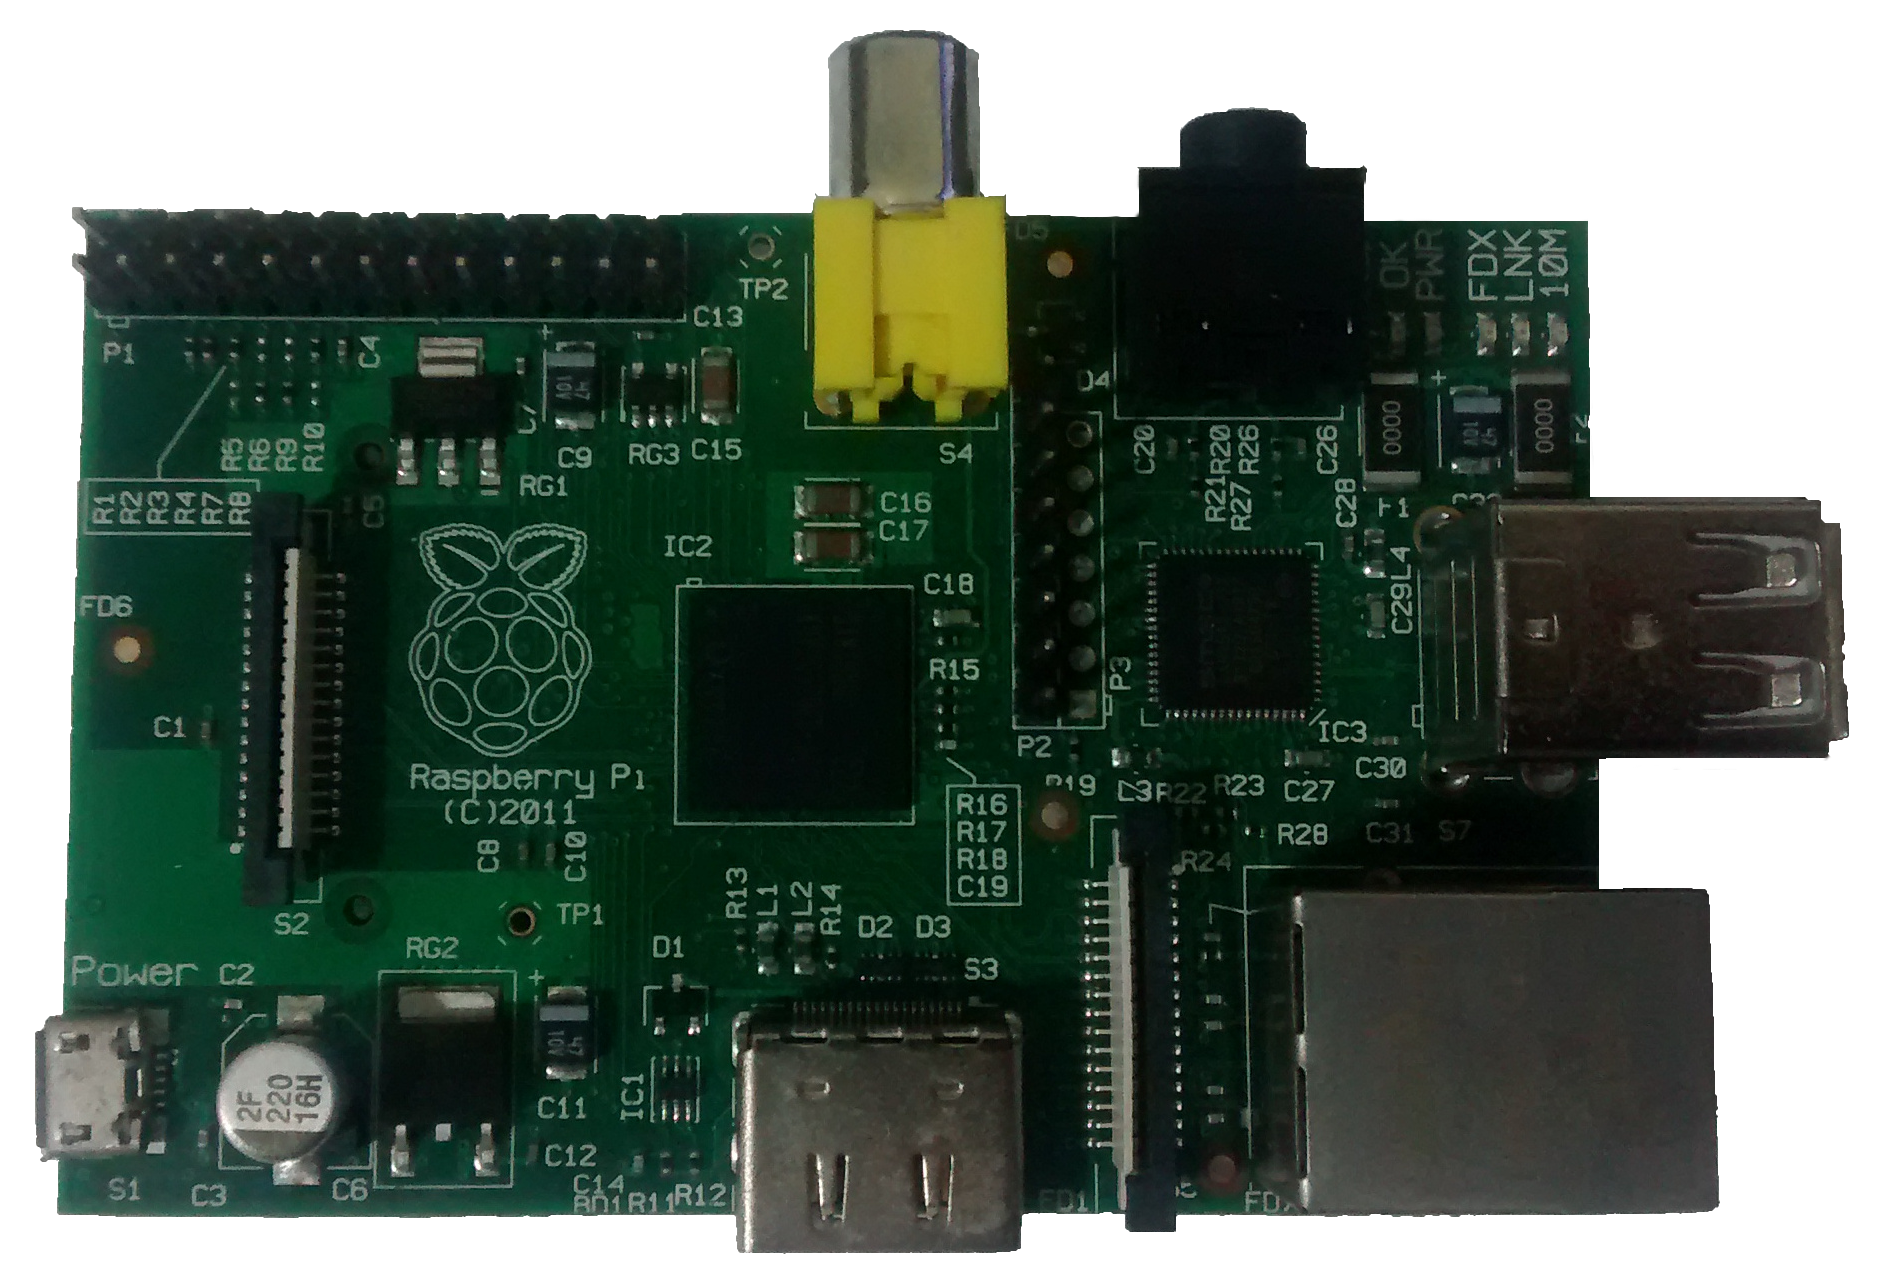
\includegraphics[width=300]{../images/raspberry.png}
	\caption{Modelo de Raspberry Pi}
	\label{figura:pi}
\end{figure}

\subsection{Sensores e Atuadores}
São as verdadeiras interfaces para o mundo físico, ou seja, são dispositivos que podem observar ou controlar
parâmetros físicos do ambiente \cite{karl_willig2005}.

Para \citeonline{fraden2010}, o propósito de um sensor é receber algum tipo de propriedade física como
entrada e convertê-la para um sinal elétrico que seja compatível com circuitos eletrônicos. Já um atuador
pode ser descrito como o oposto de um sensor, pois converte um sinal elétrico para algum tipo de energia,
geralmente não elétrica.

Este tópico será melhor aprofundado no Capítulo \ref{cap:3}.

\section{Desafios}
Embora a área de automação residencial avançou muito na última década, ainda existem algumas barreiras que
dificultam o desenvolvimento e gerenciamento de um sistema dessa categoria.

Para \citeonline{jiang_liu_yang2004}, existem três desafios fundamentais ao implementar um ambiente
automatizado. O primeiro consiste em desenvolver o sistema utilizando uma abordagem de planejamento e
integração desde o início, para que não ocorra adições crescentes de componentes tecnológicos sem que eles se
beneficiem da solução. O segundo problema consiste na interoperabilidade devido aos inúmeros fabricantes
existentes e a falta de um protocolo de comunicação acordado entre todos. Por último, tem-se a confiabilidade
como um dos principais critérios a ser atendidos.

Em uma pesquisa realizada por \citeonline{brush_2011} foram entrevistados 14 moradores de
residências automatizadas, e as principais barreiras encontradas por eles foram:
\begin{itemize}
	\item \textbf{Alto custo de propriedade:} custo relacionado em adquirir e manter o sistema de automação, seja
	ele monetário, de tempo gasto, ou ambos;
	\item \textbf{Inflexibilidade:} dificuldade em alterar ou adicionar componentes devido à necessidade de
	mudanças estruturais e à falta de compatibilidade entre dispositivos;
	\item \textbf{Gerenciamento precário:} o sistema deve prever futuras iterações do desenvolvimento para que
	essa barreira seja amenizada, além disso, é desejável que haja uma interface de usuário intuitiva
	para realizar procedimentos de manutenção;
	\item \textbf{Dificuldade em obter segurança:}  normalmente o nível de segurança é inversamente
	proporcional ao de comodidade, deixando os usuários na dúvida quanto algumas questões como acesso
	remoto, travamento de portas e janelas e vigilância.
\end{itemize}

Além desses, a característica pervasiva de uma automação domiciliar acarreta em alguns outros desafios, como
a necessidade de auto-adaptação devido ao dinamismo de comportamento, localização e hábitos dos usuários tal
como mudanças ambientais. A solução deve ser também capaz de lidar com um grande número de equipamentos
dinâmicos, de modo que ela seja facilmente escalável. Por fim, a facilidade de uso é uma das principais
barreiras que devem ser solucionadas a fim de popularizar cada vez mais esse tipo de automação
\cite{lalanda2010}.
